\documentclass{beamer}
\usepackage[portuguese]{babel}
\usepackage[utf8]{inputenc}
\usetheme{metropolis}
\setbeamertemplate{frame numbering}[fraction]
\usepackage{booktabs}

\title{Análise de Artigos Científicos sobre Internet das Coisas (IoT) com PLN}
\subtitle{Gustavo Henrique Trassi Ganaza \\ João Augusto da Silva Gomes \\ Yoshiyuki Fugie}
\institute{
    Universidade Estadual de Maringá \\
    Curso de Ciência da Computação \\
    Disciplina: Introdução a Inteligência Artificial \\
    Professor Dr. Wagner Igarashi
}
\date{\today}

\begin{document}

\maketitle

\section{Introdução}
\begin{frame}{Introdução}
\begin{itemize}
    \item \textbf{Objetivo:} Analisar um conjunto de 10 artigos científicos da área de Internet das Coisas (IoT), extraídos do portal IEEE Xplore, utilizando técnicas de Processamento de Linguagem Natural (PLN).
    \item \textbf{Escopo:}
    \begin{itemize}
        \item Leitura e pré-processamento de textos em formato PDF.
        \item Extração de informações estruturadas como objetivo, problema, método e contribuição de cada artigo.
        \item Identificação de tendências, termos-chave, técnicas mencionadas e direções para trabalhos futuros por meio de análises de frequência e visualização de dados.
    \end{itemize}
\end{itemize}
\end{frame}

\begin{frame}{Fundamentação Teórica}
\begin{itemize}
    \item \textbf{Processamento de Linguagem Natural (PLN):} Campo da inteligência artificial focado na interação entre computadores e a linguagem humana.
    \item \textbf{Pré-processamento de Texto:}
    \begin{itemize}
        \item \textbf{Lematização (spaCy):} Redução das palavras à sua forma base (lema) para agrupar termos com o mesmo significado.
        \item \textbf{Remoção de Stopwords (NLTK):} Exclusão de palavras comuns (ex: "o", "que", "de") que não agregam valor semântico à análise.
    \end{itemize}
\end{itemize}
\end{frame}

\begin{frame}{Fundamentação Teórica}
\begin{itemize}
    \item \textbf{Modelo Bag-of-Words:} Utilizado para representar os textos como um conjunto de palavras, permitindo a análise de frequência (unigramas) para identificar os termos mais relevantes.
    \item \textbf{Extração de Informação:} Uso de expressões regulares (regex) para buscar e extrair sentenças-chave que descrevem o objetivo, problema, método e contribuição dos artigos.
\end{itemize}
\end{frame}

\section{Materiais e Métodos}
\begin{frame}{Materiais}
    \begin{itemize}
        \item \textbf{Artigos Científicos:} 10 artigos selecionados do portal IEEE Xplore, focando em temas relevantes de IoT.
        \item \textbf{Ferramentas e Bibliotecas:}
        \begin{itemize}
            \item Python: Linguagem de programação.
            \item PyPDF2 e spaCy: Para extração de texto limpo e pré-processamento (lematização, tokenização).
            \item NLTK: Para remoção de stopwords.
            \item Pandas: Para manipulação e organização dos dados extraídos.
            \item WordCloud e Matplotlib: Para a geração das visualizações de dados (nuvem de palavras, gráficos).
        \end{itemize}
    \end{itemize}
\end{frame}

\begin{frame}{Artigos}
    \begin{table}
    \centering
    \footnotesize
    \begin{tabular}{|p{8cm}|c|}
        \hline
        \textbf{Título do Artigo} & \textbf{Ano} \\
        \hline
        A simplified approach for dynamic security risk management in connected and autonomous vehicles & 2019 \\
        \hline
        Automation in Agriculture and IoT & 2019 \\
        \hline
        Cloud for IoT - A survey of technologies and security features of public cloud IoT solutions & 2019 \\
        \hline
        Developing complex services in an IoT ecosystem & 2015 \\
        \hline
        Emerging privacy challenges and approaches in CAV systems & 2019 \\
        \hline
        IoT Challenges and Issues in Indian Perspective & 2018 \\
        \hline
        Next Generation Lightweight Cryptography for Smart IoT Devices Implementation Challenges and Applications & 2019 \\
        \hline
        Secure - zero touch device onboarding & 2019 \\
        \hline
        Towards an integrated privacy protection framework for IoT Contextualising regulatory requirements with industry best practices & 2019 \\
        \hline
        Towards an understanding of emerging cyber security threats in mapping the IoT & 2019 \\
        \hline
    \end{tabular}
    \end{table}
\end{frame}

\begin{frame}{Metodologia Aplicada}
    \begin{enumerate}
        \item Leitura e Limpeza: Extração de texto dos PDFs, removendo cabeçalhos e rodapés recorrentes.
        \item Pré-processamento: Aplicação de lematização e remoção de stopwords.
        \item Análise de Frequência: Contagem de unigramas para identificar os termos mais citados.
        \item Extração de Informações: Aplicação de padrões (regex) para identificar as seções de interesse.
        \item Visualização: Geração de gráficos e nuvens de palavras para ilustrar os resultados.
    \end{enumerate}
\end{frame}

\section{Resultados}
\begin{frame}{Análise Geral de Termos}
    \begin{figure}
        \centering
        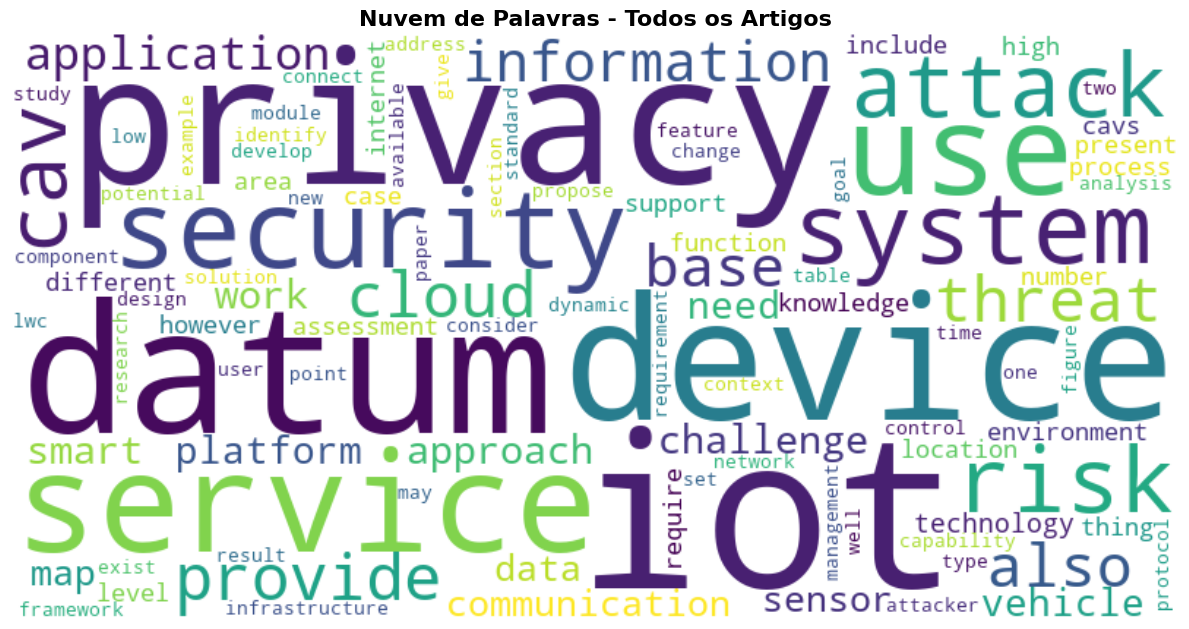
\includegraphics[width=\textwidth]{img/nuvem-palavras.png}
    \end{figure}
\end{frame}

\begin{frame}{Análise Geral de Termos}
    \begin{itemize}
        \item A nuvem de palavras destaca os termos mais frequentes em todos os artigos, fornecendo uma visão geral dos principais focos de pesquisa.
        \item Termos como "iot", "privacy", "data", "device" e "security" são os mais proeminentes, indicando que a segurança e a privacidade de dados em dispositivos IoT são os temas centrais dos artigos analisado.
    \end{itemize}
\end{frame}

\begin{frame}{Análise Geral de Termos}
    \begin{table}
    \centering
    \begin{tabular}{|c|c|}
        \hline
        \textbf{Termo} & \textbf{Frequência} \\
        \hline
        iot & 350 \\
        privacy & 248 \\
        datum & 237 \\
        device & 219 \\
        service & 216 \\
        use & 173 \\
        security & 159 \\
        system & 157 \\
        risk & 129 \\
        attack & 121 \\
        \hline
    \end{tabular}
    \end{table}
\end{frame}

\begin{frame}{Técnicas e Métodos Mencionados}
    \begin{figure}
        \centering
        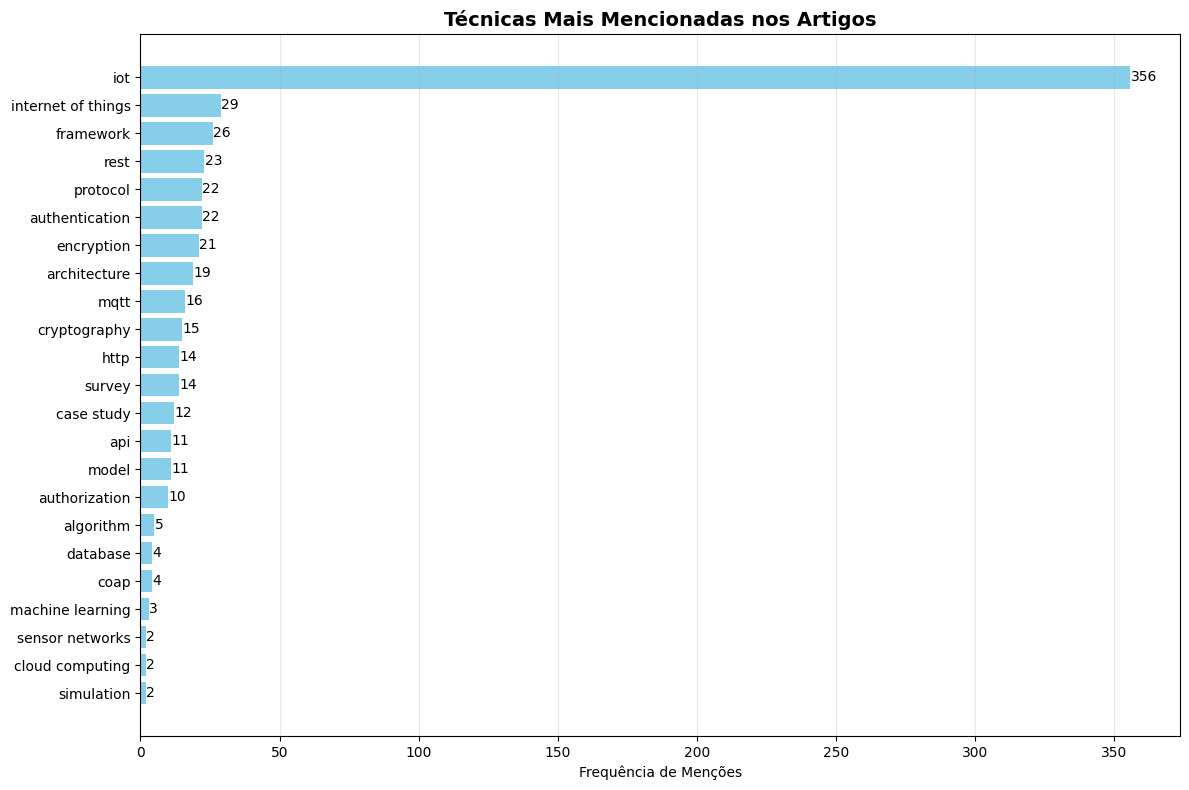
\includegraphics[width=\textwidth]{img/tecnicas-mais-mencionadas.png}
    \end{figure}
\end{frame}

\begin{frame}{Técnicas e Métodos Mencionados}
    \begin{itemize}
        \item A análise das técnicas revela um forte foco em aspectos de comunicação e segurança.
        \item Termos como "iot", "authentication", "rest" (protocolo de API), "mqtt" (protocolo de mensagens) e "encryption" aparecem com alta frequência.
        \item Isso sugere que os artigos tratam primariamente da arquitetura e da proteção de ecossistemas IoT, em vez de focar em técnicas de análise de dados como "machine learning" ou "deep learning", que tiveram menções menos expressivas no conjunto de artigos.
    \end{itemize}
\end{frame}

\begin{frame}{Técnicas e Métodos Mencionados por Artigo}
    \begin{figure}
        \centering
        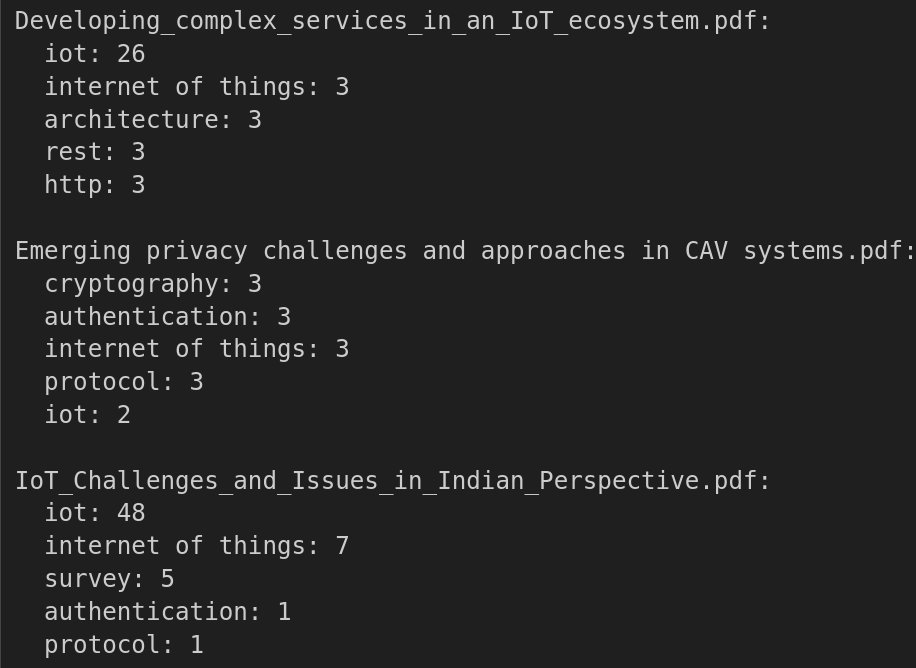
\includegraphics[width=\textwidth]{img/exemplo-tecnica.png}
    \end{figure}
\end{frame}

\begin{frame}{Evolução Temporal dos Termos}
    \begin{figure}
        \centering
        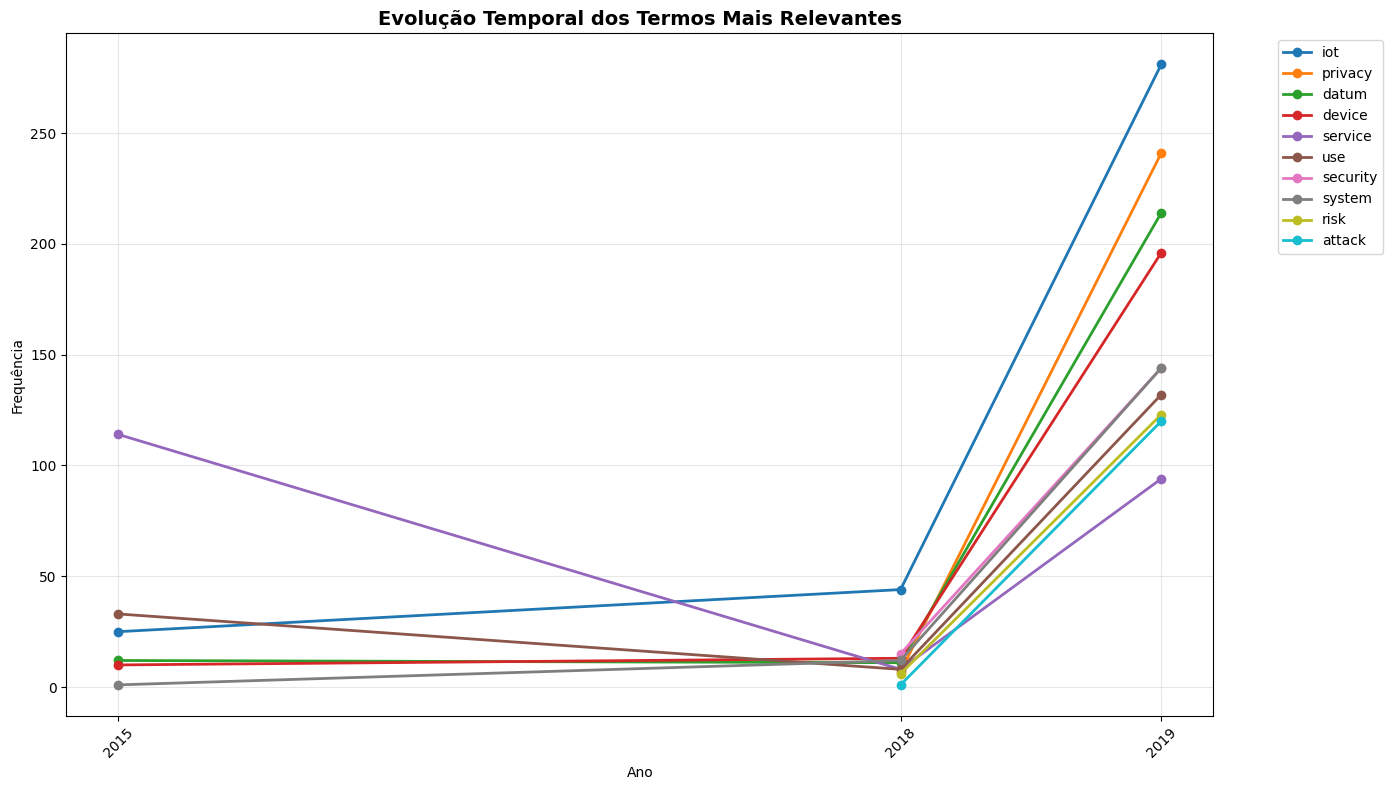
\includegraphics[width=\textwidth]{img/evolucao-temporal.png}
    \end{figure}
\end{frame}

\begin{frame}{Evolução Temporal dos Termos}
    \begin{itemize}
        \item O gráfico ilustra a frequência dos termos mais relevantes ao longo dos anos dos artigos publicados (2015, 2018, 2019).
        \item Nota-se uma alta concentração de artigos em 2019, ano em que termos como "iot", "privacy" e "data" atingiram seu pico de menções no conjunto de dados.
        \item No entanto, isso se deve ao fato de que a maioria dos artigos analisados é de 2019, o que pode distorcer a percepção da evolução temporal.
    \end{itemize}
\end{frame}

\begin{frame}{Tópicos para Trabalhos Futuros}
    \begin{figure}
        \centering
        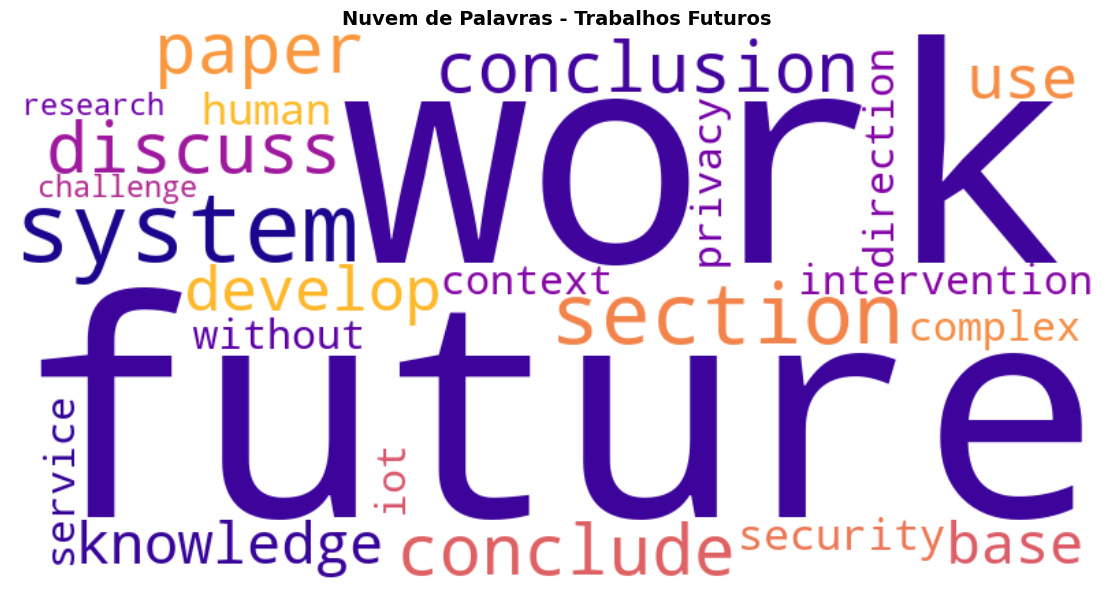
\includegraphics[width=\textwidth]{img/tabalho-futuro.png}
        \caption{Nuvem de palavras que foram identificadas como tópicos para trabalhos futuros nos artigos analisados.}
    \end{figure}
\end{frame}

\begin{frame}{Tópicos para Trabalhos Futuros}
    \begin{itemize}
        \item Foram encontrados Trabalhos Futuros em 8 artigos.
        \item Nessses 8 artigos, foram identificadas 14 sentenças que descrevem possíveis direções para pesquisas futuras.
        \item Analisando essas sentenças, percebe-se que as pesquisas apontam para a continuidade no desenvolvimento de sistemas, segurança e abordagens baseadas em conhecimento.
    \end{itemize}    
\end{frame}

\begin{frame}{Exemplo de Sentenças Extraídas para Trabalhos Futuros}
    \begin{itemize}
        \item " We anticipate that some of our future  work will be  to develop more uses of the knowledge-based  system on the security analysis, and to extend this res earch in simulation environment for further ve..."
        \item "This work categorises the emerging privacy challenges and solutions for CAV systems and identifies the knowledge ga p for future research, which will minimise and mitigate privacy concerns without ham..."
    \end{itemize}
    
\end{frame}

\begin{frame}{Conclusão}
    \begin{itemize}
        \item A análise dos artigos científicos sobre IoT revelou um foco significativo em segurança, privacidade e comunicação entre dispositivos.
        \item As técnicas de Processamento de Linguagem Natural (PLN) foram eficazes para extrair informações relevantes e identificar tendências na literatura.
        \item A evolução temporal dos termos sugere um aumento do interesse em temas relacionados à segurança e privacidade nos últimos anos.
        \item Os tópicos para trabalhos futuros indicam uma continuidade nas pesquisas, com ênfase em segurança, desenvolvimento de sistemas e abordagens baseadas em conhecimento.
    \end{itemize}
\end{frame}

\begin{frame}{Referências}
\footnotesize
\begin{itemize}
    \item \textbf{spaCy.} Industrial-Strength Natural Language Processing. Disponível em: \url{https://spacy.io/}
    \item \textbf{NLTK Project.} Natural Language Toolkit. Disponível em: \url{https://www.nltk.org/}
    \item \textbf{PyPDF2.} A pure-python PDF library. Disponível em: \url{https://pypdf2.readthedocs.io/}
    \item \textbf{WordCloud.} A little word cloud generator in Python. Disponível em: \url{https://github.com/amueller/word_cloud}
    \item \textbf{Python re module.} Regular expression operations. Disponível em: \url{https://docs.python.org/3/library/re.html}
    \item \textbf{IEEE Xplore Digital Library.} Disponível em: \url{https://ieeexplore.ieee.org/}
\end{itemize}
\end{frame}

\end{document}